\documentclass[10pt]{article}
\usepackage[margin=0.72in]{geometry}
\usepackage{booktabs,graphicx,array,microtype,xcolor,listings,caption,subcaption,xspace}
\usepackage[section]{placeins}
\usepackage[numbers,sort&compress]{natbib}
\usepackage[hidelinks]{hyperref}
\usepackage[nameinlink,noabbrev]{cleveref}
\graphicspath{{figures/}}
\definecolor{shade}{gray}{0.94}
\lstset{basicstyle=\ttfamily\footnotesize,backgroundcolor=\color{shade},frame=single,columns=fullflexible,breaklines=true}
\newcommand{\us}{\ensuremath{\mu\mathrm{s}}\xspace}
\newcommand{\eclass}[1]{\textsc{#1}}
\title{Reproducing and Extending ESP32 Workload Benchmarks on ESP32-C6:\\Performance and Generated-Code Evidence}
\author{Izbassar Yesbol}
\date{Technical report, September 2026}

\begin{document}
\maketitle
\begin{abstract}
\textbf{Introduction.} Plauska et al. measured five workloads in four languages on the classic ESP32. Their published results provide a historical comparison for ESP32-C6, but changes in hardware, software, and protocol prevent an ISA-only interpretation. We ask how these workloads behave under a common C6 protocol and what the preserved binaries can explain.

\textbf{Methods.} We implemented CRC-32, SHA-256, Q15 FFT, binary32 FIR, and binary32 IIR in C/C++, Rust, and MicroPython. Correctness-gated runs on one ESP32-C6 produced 12,000 reproduction-oriented observations and 9,600 observations under declared performance transformations. We compared local summaries descriptively with Plauska's published aggregates and inspected exact C6 binaries alongside matched, unmeasured Xtensa and RV32IMAC reconstructions.

\textbf{Results.} At the largest input, local native CRC-32, SHA-256, and FFT means were lower than the published means, while FIR and IIR means were higher. Within C6, the C++ and Rust ordering changed by workload. Exact C6 FIR/IIR binaries call software floating-point helpers; matched Xtensa objects emit floating-point instructions. An audited Rust FFT transformation reduced the median by 22.7\% relative to its safe performance build but changed the whole kernel. The C6 SHA peripheral reduced the Mode A software time by a factor of 8.70.

\textbf{Conclusions.} The workload-dependent results and generated code support specific mechanism hypotheses, including a possible software floating-point contribution to the FIR/IIR contrast. They cannot quantify that contribution or isolate ISA effects across the two platforms. This is a single-board C6 case study with a separate historical comparator.
\end{abstract}

\section{Introduction}
The classic ESP32 integrates Xtensa LX6 cores, whereas ESP32-C6 uses an Espressif RISC-V core configured as RV32IMAC \citep{espressifESP32Datasheet,espressifESP32C6Datasheet}. Comparing published results from the former with measurements from the latter is useful, but not a controlled architecture experiment: ISA, implementation, caches, flash, board, compiler backend, SDK, runtime, and protocol can all change. We therefore use \emph{platform} for the complete measured context, \emph{ISA} for the instruction-set contract, \emph{target} for a compiler configuration, and \emph{generated code} for a particular artifact.

Plauska et al. measured C/C++, Rust, MicroPython, and TinyGo on classic ESP32 using five kernels \citep{plauska2023performance}. Their paper and repository are a directly relevant historical anchor, but several inputs, warm-ups, launchers, and MicroPython boundaries are inconsistent or incompletely recoverable. We reconstruct the comparable contract on C6 and call every Plauska comparison \emph{historical and descriptive}. Only the C6 was newly measured. Xtensa objects in this study are matched reconstructions: they show how pinned toolchains lower matched source, but neither reproduce Plauska's binaries nor supply Xtensa timing.

The work makes three contributions:
\begin{enumerate}
\item an audited, correctness-gated five-workload reconstruction with common C6 timing rules and 21,600 provenance-preserving observations;
\item exact C6 and matched reconstructed Xtensa/RV32IMAC generated-code evidence linked to workload mechanisms; and
\item a strict separation between reproduction-oriented Mode A and declared Mode B transformations, exposing workload-dependent compiler, safety, and peripheral effects.
\end{enumerate}
The novelty is this integrated evidence chain, not priority over all ESP32 language or ISA studies.

\section{Architectural Context and Engineering Lens}
Quantitative computer architecture treats performance as a measured property of a complete implementation and workload, not a synonym for ISA elegance \citep{hennessy2025quantitative,patterson2020cod}. The familiar decomposition of execution time into dynamic instruction count, cycles per instruction, and clock rate is useful here precisely because we measure only elapsed kernel time. We do \emph{not} derive cycles from nominal frequency; dynamic count, CPI, cache misses, and stalls remain unmeasured. Static disassembly can identify emitted mechanisms, but not their execution frequency or latency contribution.

RISC-V began at Berkeley in 2010 through work led by Krste Asanovi\'c, Yunsup Lee, Andrew Waterman, and David Patterson; early motivation emphasized a free, extensible research and implementation ISA \citep{asanovic2014free,patterson2017reader}. John Hennessy's role belongs to the Stanford RISC/MIPS lineage and to the quantitative methodology co-developed with Patterson, not to RISC-V co-creation. This distinction matters because the paper relies on their methodological tradition rather than a founder narrative.

Xtensa is explicitly configurable and extensible \citep{gonzalez2000xtensa}; a generic Xtensa manual \citep{cadenceXtensaISASummary} therefore cannot prove a particular ESP32 feature. Vendor records describe the classic ESP32 configuration \citep{espressifESP32Datasheet,espressifESP32TRM}. For C6, vendor records identify RV32IMAC without the standard single-precision floating-point extension \citep{espressifESP32C6Datasheet,espressifESP32C6TRM}. The current unprivileged specification defines instruction semantics \citep{riscvUnpriv2026}; exact binaries, not documentation, establish what was emitted.

Our engineering reading asks four concrete questions of each kernel: what is the representation, what is the critical loop, what memory and control operations surround it, and which abstraction costs survive compilation? This resembles performance-aware programming practice, but all academic claims rest on measured artifacts and primary architecture sources.

\begin{table}[t]
\centering\small
\caption{Evidence classes keep observations separate from interpretations.}
\label{tab:evidence}
\begin{tabular}{@{}p{0.17\linewidth}p{0.72\linewidth}@{}}
\toprule Class & Meaning \\ \midrule
\eclass{Measured} & Physical C6 timing and exact preserved C6 build evidence.\\
\eclass{Published} & Plauska aggregate values; never expanded into synthetic samples.\\
\eclass{Reconstructed} & Matched-source Xtensa/RV32IMAC static artifacts; not executed.\\
\eclass{Documented} & Vendor, ISA, ABI, or toolchain statements.\\
\eclass{Derived} & Reproducibly computed summaries, ratios, tables, and figures.\\
\eclass{Inferred} & Mechanism explanation bounded by the preceding evidence.\\
\bottomrule
\end{tabular}
\end{table}

\section{Related Work}
Plauska et al. supply the five workloads and the published classic-ESP32 baseline used here \citep{plauska2023performance}. Earlier ESP32 language comparisons also matter: Ionescu and Enescu study C and MicroPython on ESP32 and STM32 \citep{ionescu2020micropythonc}; Tan et al. compare scripting runtimes on ESP32 \citep{tan2025scripting}; and Tan and Hakala examine C and MicroPython on ESP32-C3 \citep{tan2026eventdriven}. These studies establish language and runtime precedents, but use different workload contracts.

Two studies overlap more directly with the platform question. Molano Rodr\'iguez measures classic ESP32 and ESP32-C6 using separately adapted Dhrystone implementations \citep{molano2025riscvfpga}. Embuena et al. compare C and Rust across classic ESP32, ESP32-C3, and Arm boards, measuring execution time and energy for sorting, FIR, PID, and state-machine workloads \citep{embuena2026platforms}. Neither study reconstructs Plauska's five-workload protocol on C6 or combines its three retained languages with the matched code artifacts reported here. We therefore claim neither the first physical ESP32/C6 comparison nor the first cross-architecture language comparison.

Other work explains why hardware and runtime context must remain explicit. Ariel OS evaluates embedded Rust on heterogeneous targets \citep{frank2025ariel}; Femto-Containers studies portable isolation across microcontrollers \citep{zandberg2022femtocontainers}. Lima reports a C6 cryptographic energy methodology \citep{lima2025esp32c6signatures}, whereas constrained WebAssembly work includes C6 in a different runtime setting \citep{has2025wasmiot}. Our measurements address execution time and generated code. Energy, scheduling, and virtual-machine behavior remain outside their scope.

\section{Research Questions and Scope}
\textbf{RQ1.} What generated-code differences are observed between exact measured C6 RV32IMAC artifacts and matched reconstructed classic-ESP32 Xtensa artifacts, and which documented target mechanisms are consistent with C6 observations and published historical direction?

\textbf{RQ2.} Under a reconstructed common protocol, how do C/C++, Rust, and MicroPython compare within the measured C6, and how do those local results differ descriptively from Plauska's aggregates?

Mode B asks how each native language's declared performance profile changes local timing, and what the dedicated C6 SHA peripheral changes relative to frozen software. It does not equate optimizer levels or call hardware SHA an ISA feature.

\section{Methodology}
\subsection{Design, board, and controls}
This is a single-board C6 case study plus historical comparison and matched static-code analysis. The physical target was one ESP32-C6 revision 0.2 module on an ESP32-C6 Relay X1 carrier with 4 MB DIO flash at 80 MHz. The high-performance CPU was fixed and read back at 160 MHz. Dynamic frequency scaling, sleep, Wi-Fi, BLE, and IEEE 802.15.4 were disabled. Supply, ambient conditions, between-day variability, and board-unit variability were not controlled. A KWS-V20 USB meter cannot isolate module/chip rail energy; no energy result is reported.

Native timing uses \texttt{esp\_timer\_get\_time()}; MicroPython uses \texttt{time.ticks\_us()}. A resolution pilot selected repeated-kernel batches for short calls. Every raw row retains batch count, total duration, and normalized per-call time. Serial output, allocation, slicing/copying, table construction, GC preparation, validation, and cleanup lie outside the timed kernel. Small inputs principally reveal fixed/timer overhead and are not treated as throughput.

\subsection{Mode A contract}
Mode A is fair and reproduction-oriented. Each language uses the same recovered algorithm, canonical input, eight sizes (0, 16, 32, 64, 128, 256, 512, and 1024 workload units), correctness requirements, one unmeasured warm-up, and 100 accepted observations per size. CRC is CRC-32/ISO-HDLC; SHA is frozen software SHA-256; FFT preserves Q15 complex representation and scaling; FIR/IIR preserve binary32 coefficients, operation order, initial state, and tolerances. Independent host or MATLAB oracles pass before timing. C6-specific optimization and the SHA accelerator are prohibited.

The 12,000 observations are $5\times3\times8\times100$ sequential repetitions. They characterize one acquisition, not 100 independent devices or sessions. Historical audit classes recovered properties as exact, equivalent, deviation, or unknown. Inconsistent historical warm-up descriptions, MicroPython preparation, launcher iteration behavior, and validation coverage remain limitations rather than a third mode.

\subsection{Mode B contract}
Mode B retains workload semantics while declaring transformations. C++ uses ESP-IDF v5.5.5's performance configuration (GCC 14.2.0 \texttt{-O2}); Rust uses rustc/cargo 1.97.1 release opt-level 3 with \texttt{esp-idf-sys} 0.37.2. These are language-specific policies, not equivalent treatments. \texttt{HW\_SHA} times the full one-shot \texttt{mbedtls\_sha256} path, including setup/finalization, arbitration, DMA, and HAL. \texttt{RUST\_UNCHECKED} was allowed after frozen FFT preconditions proved all indexes valid; it changes checks, control flow, layout, and register allocation, so it is a whole-transformation result. CRC IRAM placement was rejected for lack of a prior fetch/cache hypothesis. Mode B contains 9,600 observations.

\subsection{Validation, statistics, and artifacts}
C++ used ESP-IDF v5.5.5/GCC 14.2.0; Rust used rustc/cargo 1.97.1 and \texttt{esp-idf-sys} 0.37.2; MicroPython used ESP32\_GENERIC\_C6 v1.28.0 (2026-04-06). Run captures record target, versions, configuration, vectors, timer, batch, board, flash, radios, correctness, and artifact hashes; the normalized one-context-row, per-observation, manifest bundle form is implemented for the CRC-32 and SHA-256 Mode A acquisitions, while the later workloads and Mode B retain the same metadata in console captures and processed run-metadata tables. Exact measured native artifacts are retained except the accepted Mode A Rust CRC ELF; that case is labelled pinned-source reconstruction.

Processing checks row counts, correctness, unique size/iteration keys, metadata, and reconstruction of normalized time. We report mean, median, sample SD, percentiles, IQR, range, and coefficient of variation. No confidence interval is presented as board-population uncertainty. Cross-study ratios use published mean/local mean because only aggregates exist; within-C6 and Mode B ratios use medians. A ratio near one is not an equivalence test.

Static disassembly records symbol size, instruction rows, loads, stores, branches, calls, stack frames, helpers, and panic references. Counts are static properties, not dynamic instructions, path frequencies, cycles, stalls, or cache misses.

\section{Mode A Results}
\begin{table}[t]
\centering\scriptsize
\caption{Largest-input local C6 medians. The language-consistent historical/local matrix is in the supplement; cross-study ratios appear in \cref{fig:historical}.}
\label{tab:headline}
\begin{tabular}{@{}lrrrr@{}}
\toprule
Workload & C++ med. & Rust med. & MicroPython med. & Published C++ mean \\
 & \multicolumn{4}{c}{Time (\(\mu\)s)} \\
\midrule
CRC-32 & 104.000 & 72.000 & 25078 & 117.630 \\
SHA-256 & 670.000 & 711.000 & 596238 & 701.090 \\
FFT (Q15) & 1185.562 & 1493.750 & 241504 & 1821.500 \\
FIR (binary32) & 188774 & 186340 & 4157999 & 30055 \\
IIR (binary32) & 3268.000 & 3277.500 & 84702 & 214.320 \\
\bottomrule
\end{tabular}

\end{table}

\Cref{fig:historical} reports the cross-study ratio of published mean to local C6 mean. Values above one mean a lower local mean. C++ ratios are 1.134 (CRC), 1.046 (SHA), 1.536 (FFT), 0.159 (FIR), and 0.066 (IIR); Rust ratios are 1.578, 1.403, 2.360, 0.130, and 0.076. The direction reversal for native binary32 kernels motivates mechanism analysis but does not identify arithmetic class or ISA as a cause.

\begin{figure}[t]
\centering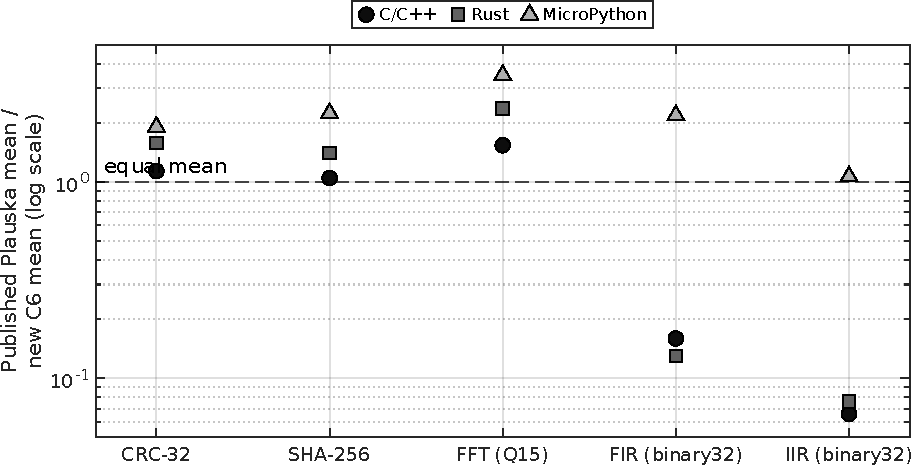
\includegraphics[width=\linewidth]{mode_a_historical_local.pdf}
\caption{Published Plauska mean divided by new physical C6 mean at the largest common input (log scale). Sources are different experiments; ratios are descriptive.}
\label{fig:historical}
\end{figure}

Within C6, ordering also varies (\cref{fig:language}). CRC medians are 104\,\us for C++ and 72\,\us for Rust (Rust/C++ 0.692). SHA gives 670 and 711\,\us (1.061). FFT gives 1185.562 and 1493.750\,\us (1.260). FIR gives 188774 and 186340\,\us (0.987), while IIR gives 3268 and 3277.5\,\us (1.003). FIR/IIR are therefore near-parity observations, not a language ranking. MicroPython is 22--890$\times$ C++ locally, but interpreter generation, numeric objects, SDK, and implementation details preclude an architectural reading.

\begin{figure}[t]
\centering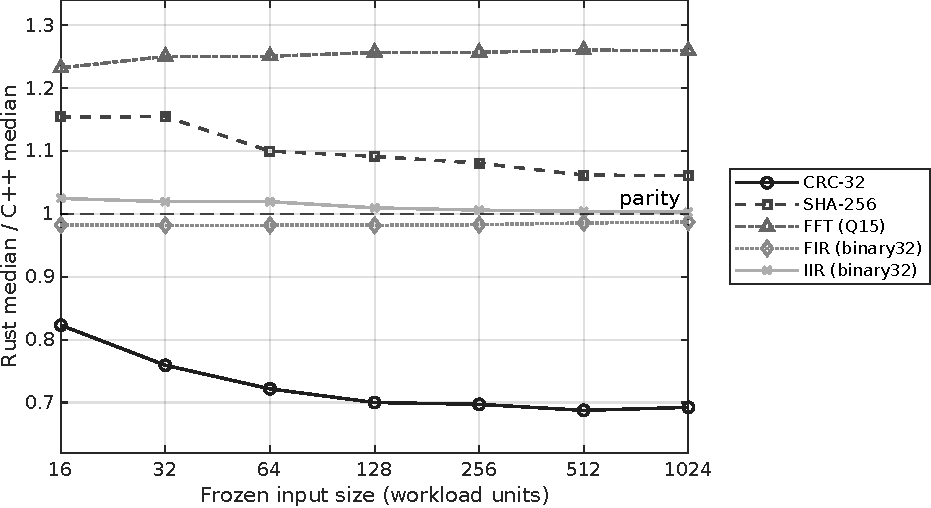
\includegraphics[width=\linewidth]{mode_a_rust_cpp.pdf}
\caption{Within-C6 Mode A Rust/C++ median ratios for nonzero frozen sizes. Size 0 remains in repository evidence but is omitted here because it primarily exposes fixed/timer overhead. Units and work differ by workload; parity is not an equivalence test.}
\label{fig:language}
\end{figure}

Largest-input within-acquisition variation is small for most native groups (for example CRC C++ mean 103.69\,\us, SD 0.884\,\us; FFT C++ mean 1185.568\,\us, SD 0.050\,\us), but says nothing about between-board or between-session uncertainty.

\section{Generated-Code Evidence}
\subsection{Integer and fixed-point kernels}
Matched CRC loops expose address formation. Xtensa uses a scaled add while RV32IMAC synthesizes it; both excerpts are copied verbatim from the matched disassemblies under \path{artifacts/assembly/crc32/cpp/}:
\begin{lstlisting}[caption={Matched CRC table addressing; static reconstruction only.}]
# matched Xtensa
addx4 a8, a8, a4
l32i.n a8, a8, 0
# matched RV32IMAC
slli a5,a5,0x2
add  a5,a5,a2
lw   a5,0(a5)
\end{lstlisting}
Matched SHA rotate idioms use Xtensa \texttt{ssai/src} versus RV32IMAC shifts and ORs. Exact Rust SHA also retains more storage/control structure than C++. These observations reveal different lowering, but no dynamic instruction count or cycle contribution.

For Q15 FFT, both targets emit scalar multiplies and shifts. No Xtensa DSP/MAC or zero-overhead-loop instruction appeared in the matched artifact. Safe Rust retains five panic references and larger control structure. The absence is a property of this binary, not evidence that Xtensa lacks such facilities.

\newpage
\subsection{Binary32 kernels and recurrence}
Exact C6 FIR contains two \texttt{\_\_mulsf3} and two \texttt{\_\_addsf3} static call sites; IIR contains five \texttt{\_\_mulsf3}, two \texttt{\_\_addsf3}, and two \texttt{\_\_subsf3}. Because the selected target has no hardware floating-point extension, binary32 arithmetic is lowered to compiler-runtime software floating-point routines \citep{gccSoftFloat1420}. Matched Xtensa FIR emits \texttt{madd.s}; matched IIR emits \texttt{mul.s}, \texttt{madd.s}, and \texttt{msub.s}. Verbatim excerpts are copied from the preserved disassemblies under \path{artifacts/builds/} and \path{artifacts/static/}:
\begin{lstlisting}[caption={Floating-point lowering, copied from the preserved disassemblies under \texttt{artifacts/builds/} and \texttt{artifacts/static/}. Call-site counts are static; reconstructed Xtensa code was not timed.}]
# exact C6 RV32IMAC
42008f0c: jalr -1184(ra) # <__mulsf3>
42008f18: jalr -1308(ra) # <__addsf3>
42008eb6: jalr -1082(ra) # <__subsf3>
# matched Xtensa reconstruction
43: madd.s f0, f2, f1
19: msub.s f1, f2, f0
\end{lstlisting}
The two strategies are not numerically equivalent in general. Xtensa \texttt{MADD.S} and \texttt{MSUB.S} perform no intermediate rounding (\citealp{cadenceXtensaISASummary} \S8.3.159, \S8.3.197), while the C6 target uses separate routines. The reconstructed and the measured kernels therefore need not agree bit-for-bit beyond the frozen tolerance.
IIR additionally has loop-carried state, constraining cross-sample reordering and lengthening the dependence chain. Compiler scheduling may differ, but the present static evidence cannot quantify its timing effect.

\section{Mode B Results}
\begin{table}[t]
\centering\small
\caption{Selected largest-input Mode B observations. Each B/A ratio uses that language's own Mode A median.}
\label{tab:modeb}
\begin{tabular}{@{}llrr@{}}
\toprule
Workload/profile & Language & Median (\(\mu\)s) & B/A \\
\midrule
CRC GCC -O2 & c\_cpp & 78.000 & 0.750 \\
CRC Rust opt-3 & rust & 77.500 & 1.076 \\
SHA GCC -O2 & c\_cpp & 626.000 & 0.934 \\
SHA Rust opt-3 & rust & 628.000 & 0.883 \\
FFT audited transform & rust & 1134.250 & 0.759 \\
SHA hardware path & c\_cpp & 77.000 & 0.115 \\
\bottomrule
\end{tabular}

\end{table}

Compiler response is not uniform (\cref{fig:compiler}). C++ CRC improves 25.0\%; C++ SHA and FIR improve about 6.6--6.7\%; C++ FFT regresses 4.9\%. Rust SHA improves 11.7\%, whereas Rust CRC regresses 7.6\%. Remaining low-single-percent changes are observations from one acquisition, not general optimizer rankings.

\begin{figure}[t]
\centering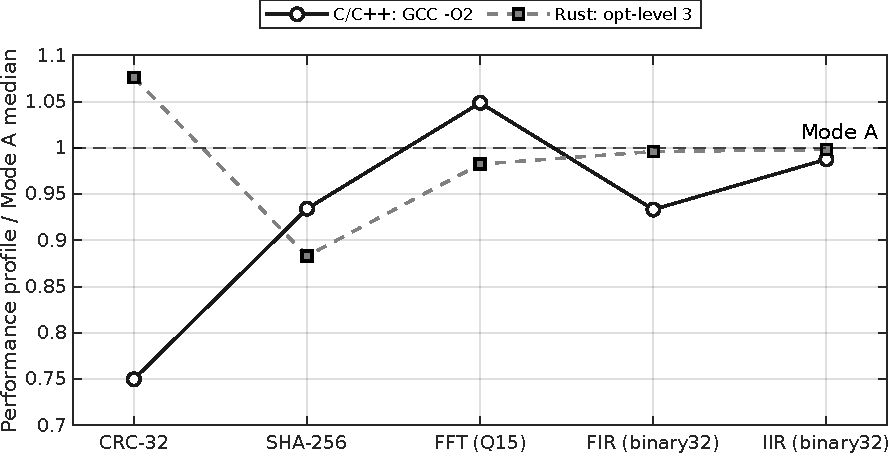
\includegraphics[width=\linewidth]{mode_b_compiler_response.pdf}
\caption{Performance-profile/Mode A median ratios. C++ \texttt{-O2} and Rust opt-level 3 are distinct policies. The clipped detail axis is explicit.}
\label{fig:compiler}
\end{figure}

The SHA hardware profile yields 77\,\us at 1024 bytes: 8.70$\times$ faster than C++ Mode A software and 8.13$\times$ faster than performance-profile software (\cref{fig:sha}). This is a complete SoC/software path, not RISC-V CPU acceleration.

\begin{figure}[t]
\centering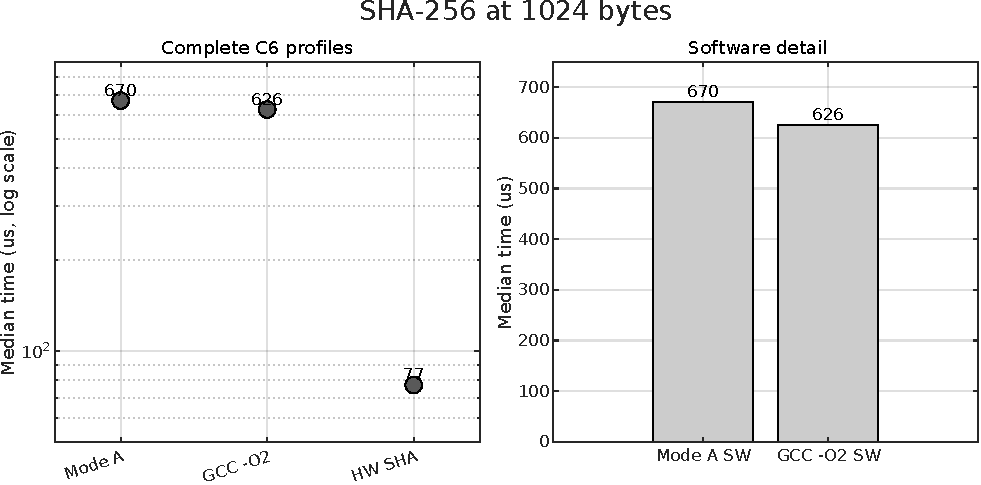
\includegraphics[width=\linewidth]{mode_b_sha_profiles.pdf}
\caption{C6 SHA-256 profiles at 1024 bytes. Left: all profiles (log scale); right: software-only zero-baseline detail.}
\label{fig:sha}
\end{figure}

Safe Rust performance FFT has 125 static instructions, 398 bytes, 18 branches, five calls, and five panic references. The audited transform has 83 instructions, 246 bytes, eight branches, no calls or panic references (\cref{tab:fft}); its median is 1134.250\,\us, 22.7\% below safe performance Rust. Since the transformation changes the entire kernel, it is not an isolated bounds-check price.

\begin{center}\small
\captionof{table}{Exact C6 Rust FFT generated-kernel profiles.}\label{tab:fft}
\begin{tabular}{@{}llrrrrr@{}}
\toprule
Kernel & Profile & Instr. & Bytes & Branches & Calls & Panic refs. \\
\midrule
FFT & Safe Rust & 125 & 398 & 18 & 5 & 5 \\
FFT & Audited transform & 83 & 246 & 8 & 0 & 0 \\
\bottomrule
\end{tabular}

\end{center}

\section{Discussion}
\paragraph{RQ1.} Target-specific contrasts appear in address formation, rotate lowering, safe control structure, and floating-point lowering. They show how matched workloads present different compiler-visible mechanisms, but not how much each mechanism contributed to Plauska's timings.

\paragraph{RQ2.} No uniform direction emerges. Local native CRC/SHA/FFT means are below published means; FIR/IIR means are above them. Within C6, Rust/C++ ordering varies and FIR/IIR are near parity. MicroPython remains much slower locally while its local means are below published means for all five kernels. Runtime and implementation changes prevent an ISA interpretation.

\paragraph{Best-supported mechanism.} \eclass{Observed}: exact C6 FIR/IIR binaries call software-FP helpers; matched Xtensa artifacts emit FP instructions; optimized C6 artifacts retain helpers; historical/native timing points in the corresponding direction. \eclass{Documented}: C6 is RV32IMAC without standard \texttt{F}, and targets without hardware floating point lower such arithmetic through compiler-runtime software routines \citep{gccSoftFloat1420}; classic ESP32 has configured floating-point facilities. \eclass{Inferred}: distinct FP execution strategies plausibly contribute materially to the historical/local FIR/IIR gap. Neither helper contribution nor pure FP-unit effect is isolated. IIR recurrence is a further plausible constraint, not a quantified cause.

Mode B reinforces interaction: native profiles help, harm, or scarcely change different kernels; the FFT source transformation changes code structure and timing; hardware SHA demonstrates a much larger peripheral opportunity while answering a different question from CPU software.

\section{Threats to Validity}
\textbf{Identification.} Only C6 was newly measured. Published classic timing, reconstructed Xtensa objects, and exact C6 artifacts are different evidence classes. Equal nominal 160 MHz neither matches microarchitecture nor establishes cycles. Compiler, SDK, runtime, board, memory, and protocol alternatives remain viable.

\textbf{Sampling.} One board and one acquisition sequence per group do not estimate board, day, supply, ambient, or session variation. One hundred repetitions characterize a sequence, not independent hardware replication. Batching and timer quantization remain in raw evidence. A C++ CRC watchdog diagnostic occurred between timed samples; rows stayed unique and correct, but it records scheduler activity outside the timing boundary.

\textbf{Construct.} Elapsed kernel time does not measure IPC, dynamic instructions, cache misses, energy, memory pressure, or application throughput. Static counts do not measure executed paths. The available USB meter cannot isolate chip energy.

\textbf{Code generation and external validity.} Matched objects were not executed; the accepted Rust CRC ELF is missing. Safe/unchecked FFT changes complete structure. Helper references and recurrence support hypotheses, not latency decomposition. One board and five compact kernels do not represent all Espressif devices, RISC-V/Xtensa implementations, toolchains, languages, or applications.

\section{Reproducibility}
The frozen experimental anchor is commit \texttt{933363b342ac960c0d364b4c6379b1ac884dec9f}. Raw evidence is immutable. Processing selects CSV columns by name, validates keys/counts/correctness/metadata, and reproduces normalized timing. MATLAB R2024b regenerates statistics and vector PDF/600-dpi PNG figures. Protocols and vectors reside under \texttt{benchmarks/historical}; Mode B under \texttt{benchmarks/optimized}; exact builds and disassemblies under \texttt{artifacts/builds} and \texttt{artifacts/assembly}. The supplement maps every claim layer to files and commands. A rerun creates a new bundle; it never overwrites accepted evidence.

\section{Future Work}
A matched physical classic-ESP32 rerun with current toolchains would strengthen platform-generation comparison, though not isolate ISA without further controls. Multiple boards, sessions, randomized profile order, supply/ambient logging, and dynamic counters would support small-effect and mechanism claims. Targeted software-FP controls could quantify helpers and dependence chains; surgical FFT variants could separate checking from induced layout changes. Precise module/chip-rail instrumentation is required for energy. WebAssembly and other languages remain separate future studies \citep{wallentowitz2022wasm,moron2023wasmjit}.

\section{Conclusion}
This ESP32-C6 extension contributes a correctness-gated physical dataset, a separated optimization campaign, preserved artifacts, and labelled matched Xtensa/RV32IMAC generated-code evidence. It is not a controlled Xtensa-versus-RISC-V performance experiment. Historical/local direction and within-C6 language ordering vary by workload. C6 FIR/IIR software helpers versus reconstructed Xtensa floating instructions form the strongest emitted-code contrast and a plausible, unquantified explanation for the binary32 direction. The Rust FFT transformation and C6 SHA peripheral expose distinct source-safety and SoC-capability effects. The supported conclusion is narrow: on this board and these frozen implementations, timing and generated structure depend on workload, language implementation, compiler profile, and platform facility; published classic-ESP32 values provide context rather than causal attribution.

\bibliographystyle{plainnat}
\begingroup\scriptsize\setlength{\bibsep}{0pt}\bibliography{references}\endgroup
\end{document}
